%% Modified by James Saunderson to comply with thesis requirements for Monash University.
%% Updated Feb 2025 to include AI statement and new cover page
%%
%% Modified by Ricardo Garcia-Rosas to satisfy the rules established by the University of Melbourne's Research Higher Degrees Committee as of 4th of June 2019.
%% Guidelines can be found at: https://gradresearch.unimelb.edu.au/__data/assets/pdf_file/0004/2027839/Preparation-of-GR-theses-rules.pdf
%%
%% ----------------------------------------------------------------
%% Thesis.tex -- MAIN FILE (the one that you compile with LaTeX)
%% ----------------------------------------------------------------

% Set up the document
\documentclass[a4paper, 11pt, oneside]{Thesis}  % Use the "Thesis" style, based on the ECS Thesis style by Steve Gunn
%
% Put your figures in this directory
\graphicspath{Figures/}  % Location of the graphics files (set up for graphics to be in PDF format)
%

% Include any extra LaTeX packages required
\usepackage[square, numbers, comma, sort&compress]{natbib}  % Use the "Natbib" style for the references in the Bibliography
\usepackage{verbatim}  % Needed for the "comment" environment to make LaTeX comments
\usepackage{vector}  % Allows "\bvec{}" and "\buvec{}" for "blackboard" style bold vectors in maths
\usepackage{miller} % formatting Miller indices
\usepackage{outlines}
\usepackage[table]{xcolor}
\usepackage{mhchem}

\hypersetup{urlcolor=blue, colorlinks=true}  % Colours hyperlinks in blue, but this can be distracting if there are many links.

%% ----------------------------------------------------------------
\begin{document}
\frontmatter      % Begin Roman style (i, ii, iii, iv...) page numbering

%
\UNIVERSITY{{Monash University}}
%
%%%%%%%%%%%%%%%%%%%%%%%%%%%%%%%%%%%%%%%%%%%%%%%%%%%%%%%%%%%%%%%%%%%%%%%%%
% Update your faculty here:
%\school{{Faculty of Engineering}}
% update your department/school here
\department{{Department of Materials Science and Engineering}}
% this is the year of submission
\gradtime{{20xx}}
% degree the thesis is for (Master of Engineering Science or Doctor of Philosophy)
\degree{xx}
%\degree{Doctor of Philosophy}
%\degree{Master of Engineering Science}

% degrees currently held by the student
%\studentdegree{B.E. (Hons), B.Sc. (Physics)}
\studentdegree{PhD Confirmation Milestone Report}
%%%%%%%%%%%%%%%%%%%%%%%%%%%%%%%%%%%%%%%%%%%%%%%%%%%%%%%%%%%%%%%%%%%%%%%%%

%
%%%%%%%%%%%%%%%%%%%%%%%%%%%%%%%%%%%%%%%%%%%%%%%%%%%%%%%%%%%%%%%%%%%%%%%%%
% Set up the Title Page
% Change your thesis title and your information here
\title  {Understanding texture effects on deformation mechanisms in Zircaloy-4}
\authors  {Ethan Sprague}

%%%%%%%%%%%%%%%%%%%%%%%%%%%%%%%%%%%%%%%%%%%%%%%%%%%%%%%%%%%%%%%%%%%%%%%%%

\maketitle
%% ----------------------------------------------------------------

\setstretch{1.3}  % It is better to have smaller font and larger line spacing than the other way round

% Define the page headers using the FancyHdr package and set up for one-sided printing
\fancyhead{}  % Clears all page headers and footers
\rhead{\thepage}  % Sets the right side header to show the page number
\lhead{}  % Clears the left side page header

\pagestyle{fancy}  % Finally, use the "fancy" page style to implement the FancyHdr headers


%% ----------------------------------------------------------------
% https://www.monash.edu/graduate-research/examination/publication
% https://www.monash.edu/rlo/graduate-research-writing/write-the-thesis
% https://www.monash.edu/rlo/graduate-research-writing/write-the-thesis/writing-the-thesis-chapters/structuring-a-long-text
\abstract{
\addtocontents{toc}{}  % Add a gap in the Contents, for aesthetics

\emph{The abstract should outline the main approach and findings of the thesis and must not be more than 500 words.}

}

\clearpage  % Abstract ended, start a new page

\pagestyle{fancy}  %The page style headers have been "empty" all this time, now use the "fancy" headers as defined before to bring them back


%% ----------------------------------------------------------------
\lhead{\emph{Contents}}  % Set the left side page header to "Contents"
\tableofcontents  % Write out the Table of Contents

%% ----------------------------------------------------------------
% End of the pre-able, contents and lists of things


%% ----------------------------------------------------------------
\mainmatter	  % Begin normal, numeric (1,2,3...) page numbering
\pagestyle{fancy}  % Return the page headers back to the "fancy" style

% Include the chapters of the thesis, as separate files
% Just uncomment the lines as you write the chapters

\fancyhead{}  % Clears all page headers and footers
\rhead{\thepage}  % Sets the right side header to show the page number
\lhead{}  % Clears the left side page header
\chapter{Introduction}

The fuel cladding for the nuclear fuel of pressurised water reactors is a critical component for which reliable integrity evaluations must be made over the entire fuel cycle, from service to waste storage.
Zirconium alloys are selected for the cladding material because of their low neutron absorption, good corrosion resistance and suitable mechanical properties.
It is crucial that the mechanical behaviour of these alloys is well understood, and accurate models are necessary for safety assessments.
Increasingly, advanced safety systems use a 'digital twin' model of the entire reactor which must accurately predict the mechanical response of the cladding material during simulated emergencies.

Zirconium alloys used for cladding have a hexagonal close packed (HCP) crystal structure.
These alloys always develop a strong crystallographic texture during conventional processing such as rolling and pilgering.
This crystallographic texture has a significant impact on the mechanical behaviour, resulting in a large anisotropy and directional dependence.
Furthermore, the texture also impacts other properties such as the formation sites for hydrides, which preferentially grow along specific crystallographic planes.
Finally, polycrystalline deformation requires each grain to accommodate the deformation of its neighbour grains, even when there is a mismatch in the single crystal properties due differences in orientation.
These neighbour interactions must be taken into account during both in-service and storage conditions, where thermal cycling and variations in pressure can lead to heterogeneous deformation.

The seemingly unavoidable crystallographic texture which emerges from processing dominates samples that are used to study the behaviour of these alloys.
Since texture has such a large effect, it is possible that underlying behaviours are being obscured by texture effects.
Material modelling should be able to accurately predict the mechanical performance of these alloys for any given texture, however, these models have only ever been extensively tested against data from strongly textured material.

This project uses powder metallurgy techniques, namely hot isostatic pressing (HIP) to create HCP material with a truly random texture by eliminating all sources of directional stress.
Studying this material alongside its conventionally processed equivalent enables a far more robust approach to optimising existing material models, with the additional constraint of a randomly textured material.

This work is directed at understanding zircaloy-4, but the results will have broader impact more generally on similar hexagonal metals such as $\alpha$-titanium alloys.
The new in-situ testing capabilities at Monash Centre for Electron Microscopy provide the opportunity to understand the complex and asymmetric deformation within these hexagonal polycrystalline materials, allowing for a deeper understanding on fundamental deformation of an entire class of alloys.
Finally, this project opens the pathway for future study on other texture-related phenomenon such as the effect of hydrides in texture-free material. % Introduction

\chapter{Literature review}

\section{Deformation modes}
HCP metals, such as $\alpha$ titanium and zirconium, exhibit complex plastic deformation behaviour which is a direct consequence of the intrinsic anisotropy of their low-symmetry crystal structure.
In contrast to FCC metals which have 12 independent and evenly distributed slip systems which can facilitate homogenous deformation for any arbitrary shear, HCP metals rely on a more restricted set of slip systems with widely varying critical resolved shear stresses (CRSS).
Many of the HCP slip systems are not independent, meaning the shear strain that they provide can be equivalently facilitated by a linear combination of other slip systems.
The Von-Mises criterion states that 5 independent slip systems are required to facilitate homogenous arbitrary deformation.
In order to satisfy this condition in HCP, more complex modes such as difficult pyramidal $\langle c + a \rangle$ or deformation twinning must be activated.

\begin{figure}[h!]
\centering
  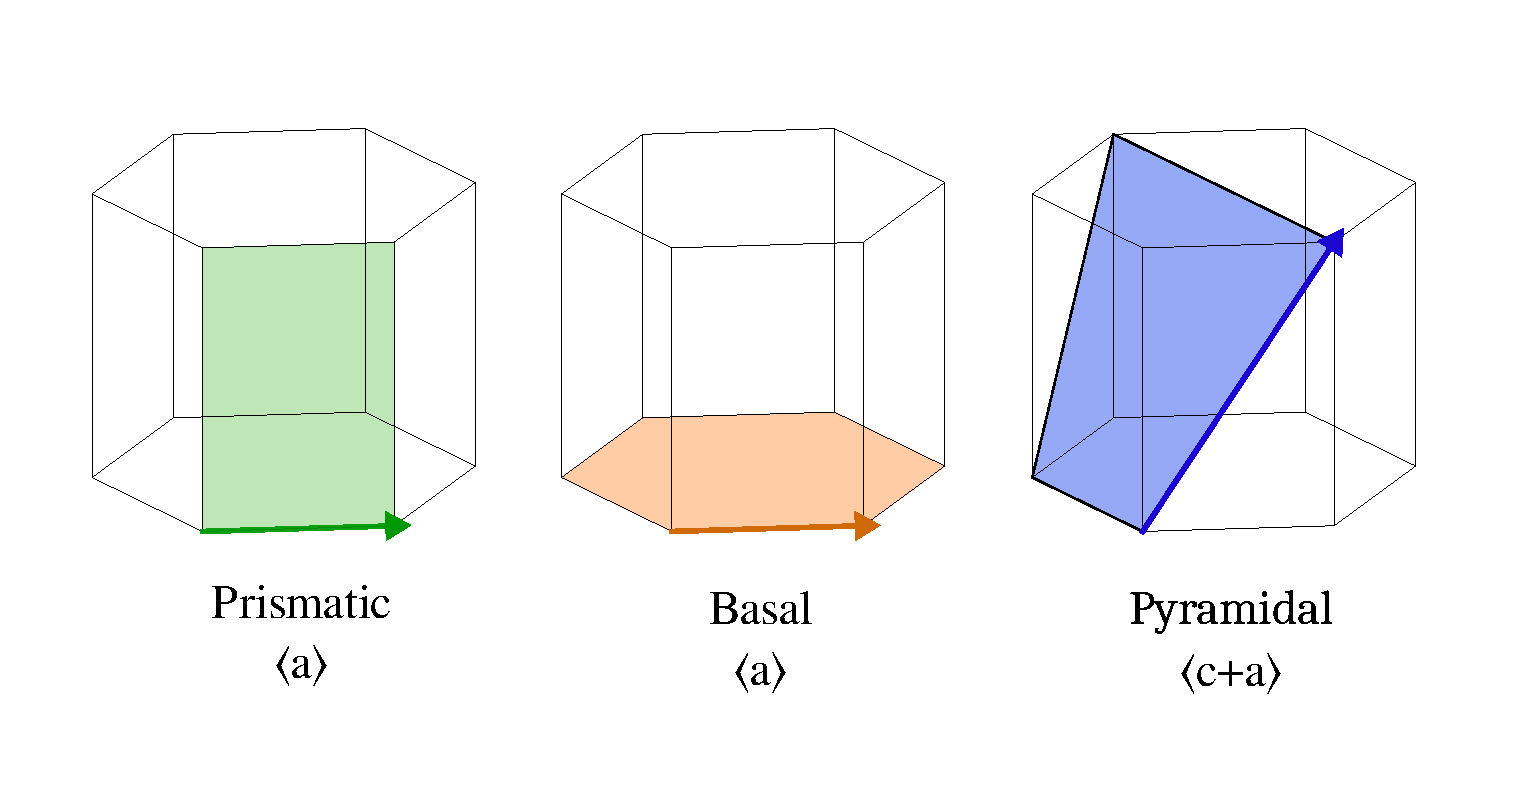
\includegraphics[width=\textwidth]{Figures/slip_systems.pdf}
  \caption{Dominant slip modes in hcp metals.\label{fig.hcp-deformation}}
  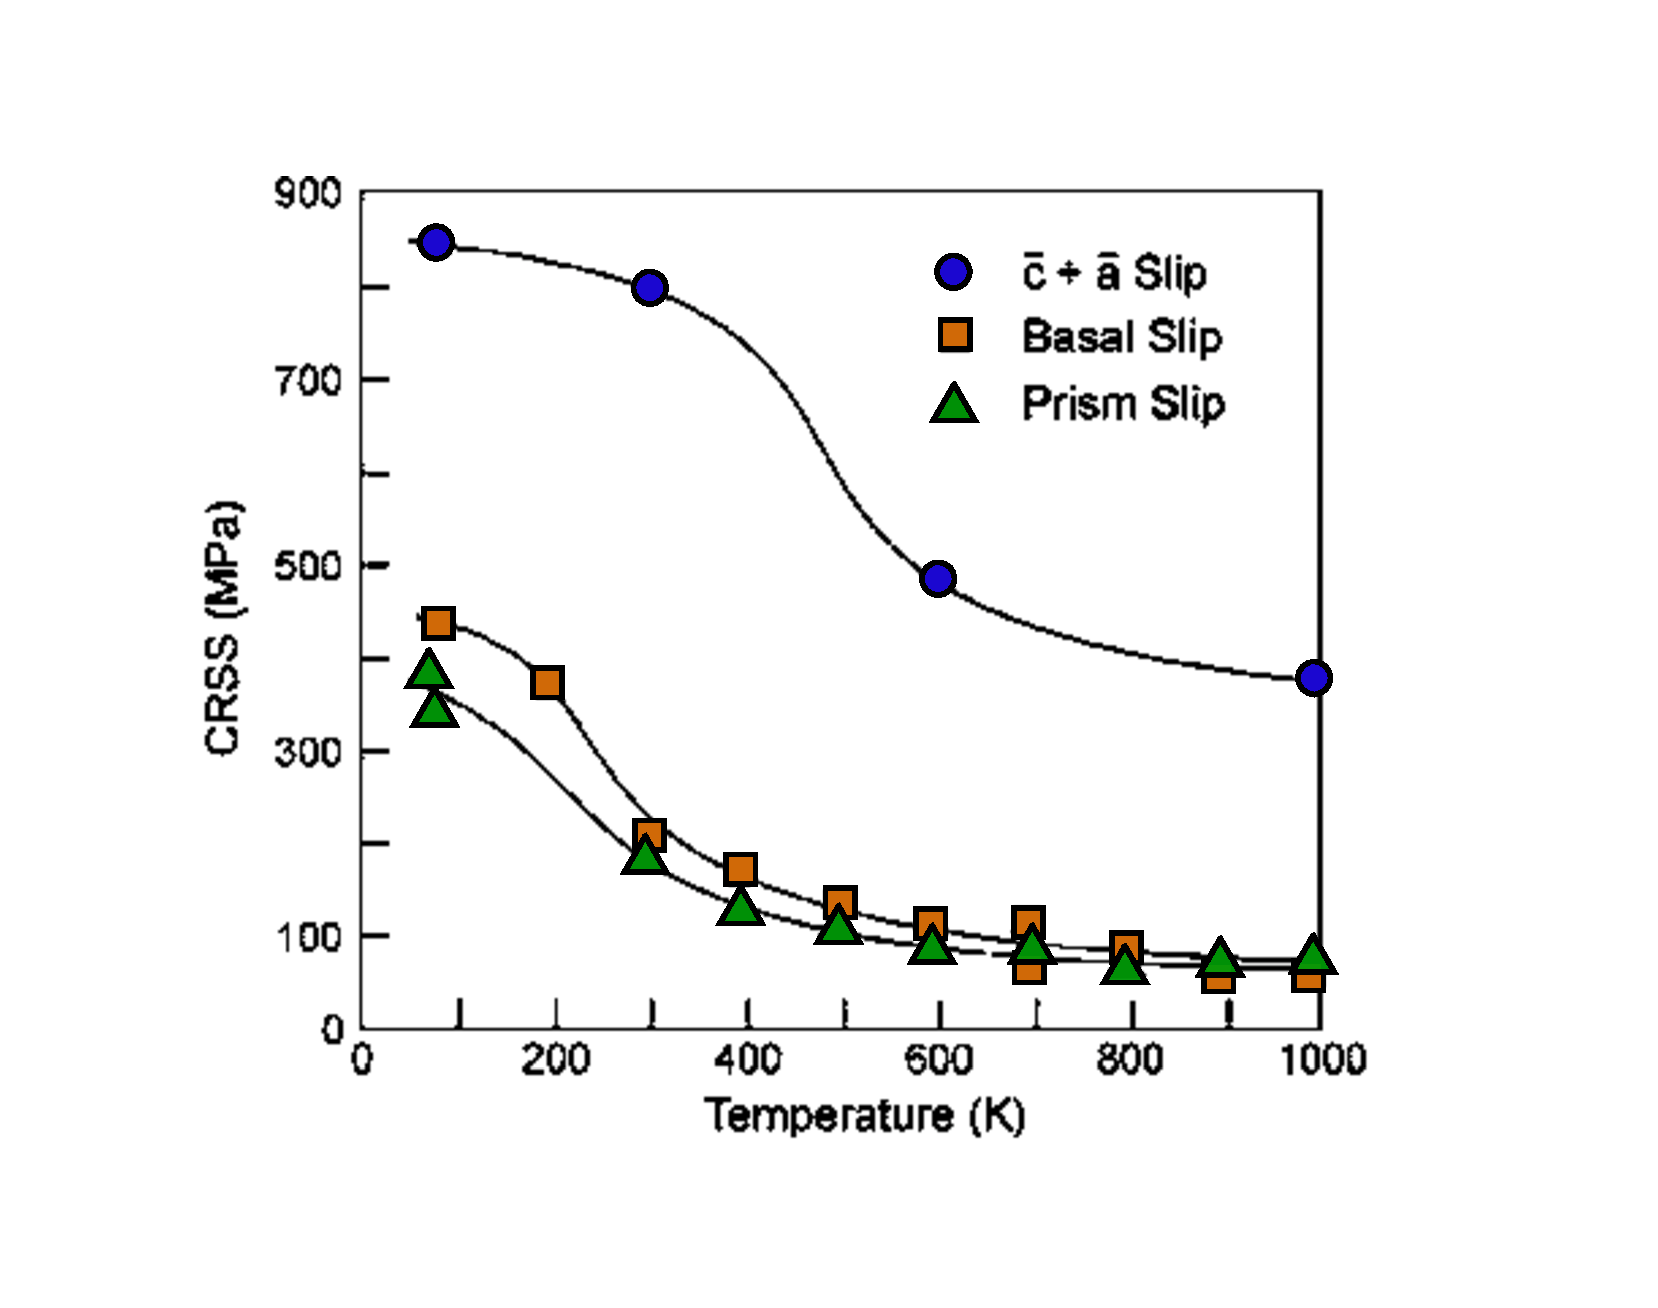
\includegraphics[width=\textwidth]{Figures/CRSS_plot.pdf}
  \caption{Critical resolved shear stresses in Ti-6.6Al single crystal\cite{lütjering2013titanium}.\label{fig.CRSS} }
\end{figure}

\subsection{Slip}
The most favourable slip occurs along crystal planes with the highest atomic packing density.
For a HCP structure with an ideal $c/a$ ratio, this would be the basal \hkl(0002) plane, however in both titanium and zirconium the $c/a$ ratio is less than the ideal value of 1.633, being 1.587 and 1.593 respectively.
This compacted HCP structure results in the highest atomic density on the prismatic planes \hkl{1 0 -1 0}, followed closely by the basal plane \hkl(0002).
The slip direction on both of these planes occurs along the $\langle a \rangle$ direction \hkl<1 1 -2 0>.
Because the Burgers vector of both of these slip families is shared, they cannot provide any shear strain that has a $\langle c \rangle$-axis component.
If one considers a loading along the $\langle c \rangle$-axis, the Schmid factor for both basal and prismatic slip would be zero, meaning plastic deformation must come from another slip mode from a plane that necessarily has a lower atomic density.
The slip mode that activates in this case is the pyramidal $\langle c + a \rangle$, on the \hkl{1 0 -1 1} plane along the \hkl<1 1 -2 3> direction which is the sum of the $\langle c \rangle$ and $\langle a \rangle$ basis vectors.
\fref{fig.CRSS} compares the CRSS values for these three major slip modes as a function of temperature in a Ti-6.6Al single crystal. 
The vast difference in CRSS between the $\langle a \rangle$ and $\langle c + a \rangle$ slip modes results in the heavily anisotropic plastic behaviour of HCP metals.
The crystal orientation of a grain therefore becomes one of the most important factors determining how it will deform, since this will dictate which of the slip modes will be active and what the resolved shear stress will be.



\subsection{Twinning}
Deformation twinning offers an alternative way for the crystal structure to accommodate $\langle c \rangle$-axis strain and is often the favourable mode due to the high CRSS of pyramidal $\langle c + a \rangle$ slip.
The available twinning modes are listed in \tref{table.twin-modes}, which are classified into tensile and compression type twins based on the $\langle c \rangle$ component of the shear.
Twinning is a coordinated reorientation of the lattice and has a distinct orientation relationship with the parent crystal, which can be defined in terms of an angle-axis representation, also listed in \tref{table.twin-modes}.
All of these twin modes result in a tilting of the $\langle c \rangle$-axis, this means that the resulting crystal within the twin volume will be quite distinct from its parent material in terms of plastic response.
For example, for loading along the $\langle c \rangle$-axis a grain will initially be quite hard. If the Type I tensile twin activates, the resulting region will have its $\langle c \rangle$-axis tilted by 85°, resulting in quite a soft orientation that is well aligned for prismatic slip.

%\ Table of twinning modes and their 
\begin{table}[h]
  \vspace{\baselineskip}
  \centering
  \begin{tabular}{l c c c}
    \hline
    \rowcolor{gray!10}
    \textbf{Twinning mode} & $\mathbf{K_1}$   & \textbf{Angle – axis}                       & $\varepsilon$ \\
    \hline
    Tensile Type I         & $\{10\bar{1}2\}$ & $85^\circ \langle 11\bar{2}0 \rangle$       & 0.171         \\
    Tensile Type II        & $\{11\bar{2}1\}$ & $35^\circ \langle 1\bar{1}00 \rangle$       & 0.629         \\
    Compression Type I     & $\{11\bar{2}2\}$ & $65^\circ \langle 1\bar{1}00 \rangle$       & 0.221         \\
    Compression Type II    & $\{10\bar{1}1\}$ & $54^\circ \langle \bar{1}2\bar{1}0 \rangle$ & 0.101         \\
    \hline
  \end{tabular}
  \caption{Twinning systems with twin plane, axis-angle representation, and twinning shear $\varepsilon$. (Nervo. 2016)}
  \label{table.twin-modes}
\end{table}

Unlike slip, deformation twinning has limited activity and eventually becomes exhausted.
In HCP metals, twinning occurs in the early stages of plasticity where it plays a large role in accommodating $\langle c \rangle$-axis strain in grains that are poorly aligned for prismatic slip.
After twin nucleation and growth, eventually the twins consume the majority of their initial grains and subsequent plasticity can continue through dislocation slip.

Deformation twinning adds to the complexity of HCP metals since twin boundaries act as barriers to dislocation motion and secondary twins can form within the primary twin volume.
An accurate description of the deformation behaviour of HCP metals must take all of this into account.

\section{Texture development}
Conventional processing of HCP alloys always produces strong crystallographic texture.
In the case of $\alpha$-titanium and zirconium which have a similar $c/a$ ratio, the particular texture that develops during cold rolling is a basal texture with a split toward the transverse direction of $\pm 25-35^\circ$.
Texture develops during cold working because of the significant crystallographic reorientation that is associated with deformation twinning.
The roller imposes a compressive stress normal to the plane of the plate, but due to the Poisson effect there is a tensile stress in the plane of the plate.
Both compressive (Type I) and tensile (Type I and II) twins have been observed to activate under cold rolling conditions \cite{bozzoloMisorientationsInducedDeformation2010}.
The twinning activity during the early stages of plasticity cause a significant initial texture change, and then subsequent plastic slip may cause further crystallographic reorientation.
Unlike twinning which causes an immediate reorientation, slip results in a gradual rotation.
Prismatic slip, which is the most active slip mode, results in a rotation about the $\langle c \rangle$-axis, while basal and pyramidal $\langle c + a \rangle$ cause the $\langle c \rangle$-axis to tilt.

The final texture that is present after cold rolling is inherited by the recrystallised microstructure, possibly due to preferential nucleation within the twinned regions.
The exact processing route and parameters effect the final resulting texture, but the fact remains that conventional processing of these alloys always results in a strong crystallographic texture.


\section{Polycrystal neighbourhood effects}
\subsection{Slip transfer}
\subsection{Strain networks}

\section{Crystal plasticity modelling} % Literature review 

\chapter{Research aims}

\section{Aims}
\begin{enumerate}
    \item Create texture-free HCP alloys (Ti/Zr) using HIP
    \item Inform crystal plasticity model with mechanical testing results
    \item Gain deeper understanding of fundamental deformation behaviour, especially polycrystal neighbourhood effects using in-situ methods
    \item Use insights to develop novel behaviour law for crystal plasticity models
\end{enumerate}

\section{Objectives}

\textbf{HIP process:}
\begin{itemize}
    \item Determine working HIP parameters for producing desired material
    \item Consider how temperature and pressure profiles, dwell time, powder stock, can geometry, and packing density affect the final microstructure (porosity, grain size distribution)
\end{itemize}

\textbf{Perform comprehensive mechanical testing:}
\begin{itemize}
    \item Generate accurate and reliable experimental data from standard mechanical tests (tensile tests, cyclic loading, hot compression)
\end{itemize}

\pagebreak
\textbf{Inform CP-FFT model:}
\begin{itemize}
    \item Create virtual representative volume element using Dream3D, use MFront to define material behaviour law, use AMITEX to solve constitutive equations in FFT regime
    \item Perform parameter fitting using mechanical test data
    \item Evaluate model generality with respect to texture by comparing results for HIPed and conventionally processed material
\end{itemize}

\textbf{In-situ testing}
\begin{itemize}
    \item Use HR-DIC to track plastic strain during loading 
\end{itemize} 

\chapter{Methodology}

\section{Hot Isostatic Press (HIP)}
In order to produce random-texture HCP metal, commercially pure titanium powder was consolidated into a bulk solid using hot isostatic pressing.
Three different powder stocks were available for this project, all grade 2 titanium but with different powder particle size distributions.
These size distributions were listed as $15-53\mu\textnormal{m}$, $45-90\mu\textnormal{m}$, and $50-150\mu\textnormal{m}$.
The powder was packed into a cylindrical stainless steel can, which had internal diameter of 50mm and internal height of 120mm.
A bottom and a top cap were welded to the cylindrical casing, with the top tube including a small filling tube to allow insertion of the powder.
The powder packing was done by hand using a funnel. Shaking and knocking the outside of the can to condense the powder resulted in a good packing density which was estimated to be ~70\% based on mass gain.

The can was evacuated through the filling tube at the top of the can over several hours to remove the gas between the powder particles.
This filling tube was then crimped and the end of the tube was welded to ensure a complete seal.
Once fully sealed, the can was placed inside the HIP chamber and the run was commenced with the following program.
Importantly, the maximum temperature during this program was measured with a thermocouple to be 854$^\circ$C which is below the expected $\beta$-transus of CP-Ti which is approximately $920^\circ\textnormal{C}$.
Staying below the beta transus is very important due to the vastly different grain boundary mobility between the alpha and beta phases.
The BCC crystal structure of the beta phase allows for much faster grain growth, which would not be ideal for studying equiaxed polycrystalline behaviour.
\pagebreak

\textbf{HIP program:}
\begin{enumerate}
    \item Evacuate to 1 torr
    \item Pump up to 100 Bar
    \item Pump up to 1500 Bar \& ramp up to 850$^\circ$C over 170 minutes 
    \item Dwell for 240 minutes
    \item Vent to 100 Bar and ramp down to 100$^\circ$C over 150 minutes
    \item Free cool to 75$^\circ$C
    \item Vent to 20 Bar
\end{enumerate}

Because of the isostatic stress condition, it was hypothesised that no preferred crystallographic orientations would exist, and therefore no texture development would occur.
The mechanisms that drive texture development during conventional processing are a response to the directionally dependent stress state, in which grains of certain orientations behave differently.
During the HIP, the plasticity that powder particles experience is dependent on the local contact points of adjacent powder particles, which can be assumed to be random.
These local stress conditions can also be assumed to be on average isostatic, meaning no orientation dependent phenomena should occur.

The major limitations associated with HIPing are the cost, time and the inability to monitor the microstructure at intermediate stages.


\section{Optical microscopy}
Optical microscopy using polarised light was used for routine microstructure characterisation.
Sample preparation involved grinding with silicon carbide paper (800, 1200, 2500 grit) followed by chemical-mechanical polishing using a mixture of 1 part \ce{H2O2}(30\%) with 4 parts OP-S using a Struers MD-Chem polishing cloth.
During the OP-S polishing step, it is important to apply pressure so that the reaction products can be mechanically removed.

The Olympus GX51 optical microscope was used for the majority of optical characterisation as it supports usage of polarising filters.
The HCP material that this project deals with (CP-Ti and Zr alloys) have an interaction with polarised light that allows for crystallographic contrast.
When these materials are viewed under cross polarisers, the intensity of reflected light depends on the orientation of the $\langle c \rangle$-axis with respect to the viewing axis.
Therefore, when a polycrystal is observed, good contrast between the grains is achieved due to differences in their crystal orientation.

This technique has limited quantitative effectiveness, it cannot determine the full crystal orientation (only the $\langle c \rangle$-axis tilt) and some other factors affect the intensity such as the surface morphology and the angle between cross polarisers.

\section{Electron Backscatter Diffraction (EBSD)}
Electron microscopy techniques can be used to acquire full quantitative information about the crystallographic orientations within samples.
This project utilises the JEOL IT800 SEM equipped with an Oxford EBSD symmetry detector.
EBSD is a very widespread technique among published literature as it offers high resolution imaging, phase mapping and grain identification.
The procedure involves mounting a small sectioned and polished sample inside the SEM stage and tilting the stage by 70$^\circ$.
The EBSD detector can then be calibrated for background corrections in order to receive a high quality signal of Kikuchi bands, which are used to identify material phases and calculate the orientation.
Electropolishing is necessary to obtain pristine sample surface quality before EBSD analysis if high resolution imaging is required.
For texture analysis, large area and low resolution imaging is sufficient.

Some care must be taken regarding the conventions for describing HCP orientations.
The oxford convention is to report the Euler angles by the Bunge convention (as passive rotations from the sample frame to the crystal frame) and defining the local X axis as being parallel to the crystal $\langle a \rangle$-axis.

For general characterisation, optical microscopy is preferred due to its time and cost efficiency, however EBSD was used when quantitative crystallographic orientation data was needed.

\section{Mechanical testing}
Cylindrical samples were machined with a gauge diameter of 3mm and gauge length of 15mm.
Uniaxial tensile tests were conducted using screw-driven Instron testing machines with a  strain rate of 0.02mm/s.
The 10kN load cell was used to maximise accuracy of the force transducer measurements, since the load on the sample was expected to reach 7kN which is outside the ideal range for the 100kN load cell.
An extensometer was attached to the sample for accurate strain measurements.

Circular samples are preferred because it is easier to obtain good alignment of the sample with the loading axis, which ensures accurate and reproducible data.
Small sample geometry was chosen in order to maximise the number of samples that could be made from a single HIP can, since the HIP runs are costly.

\section{Crystal plasticity modelling}
The modelling strategy is to build a workflow that can be easily adapted to fit many materials problems of similar nature.
The software packages that were chosen were selected to be ones that could be easily customised and compartmentalised.
This basic workflow can be divided into three main stages: material, behaviour, solver.

The simulated material that will be used for the crystal plasticity model, known as the representative volume element, is a virtual reconstruction of the polycrystalline microstructure that contains all the information about the material properties and crystallographic orientations.
In our case, this can be stored as a set of \textit{.vtk} files that represent the material information as a volume of 3-dimensional elements known as voxels.
The software package chosen for the generation and manipulation of these material files is Dream3D.
Both synthetic material construction and experimentally informed reconstruction (using EBSD data) can be done with Dream3D.

The material behaviour laws which describe the crystal plasticity behaviour explicitly can be created and compiled into machine language with the MFront library.
Here the detailed interactions between different deformation modes and their hardening behaviours can be described and tweaked.

Finally, the solver that was selected is AMITEX which is an open source project that specialises in fast fourier transform (FFT) based algorithms for solving materials modelling problems.
AMITEX has straightforward documentation detailing how to import materials and behaviour files, and also how to control the loading conditions of the simulation.
The advantage of AMITEX is its portability and customisability, as well as some unique advanced features such as composite voxels which allow for multiple behaviour laws to operate within a single material point, allowing smooth boundaries and complex interfaces to be handled properly which is one of the major struggles previously with FFT methods. 

\chapter{Research completed to date}

\section{CP-Ti plate}
Conventionally processed CP-Ti (grade 2) plate with a thickness of 8mm, and sheet with a thickness of 0.7mm, were purchased from Specialty Metals.
Both the plate and sheet had undergone a recrystallisation anneal but the exact process parameters were not reported.
Optical microscopy was used for basic microstructure characterisation, shown in \fref{fig.plateSheetOM}, and found equiaxed $\alpha$-Ti grains.
The average grain size (linear intercept) for the plate and sheet were $25\mu$m and $15\mu$m respectively.

\begin{figure}[h]
\centering
  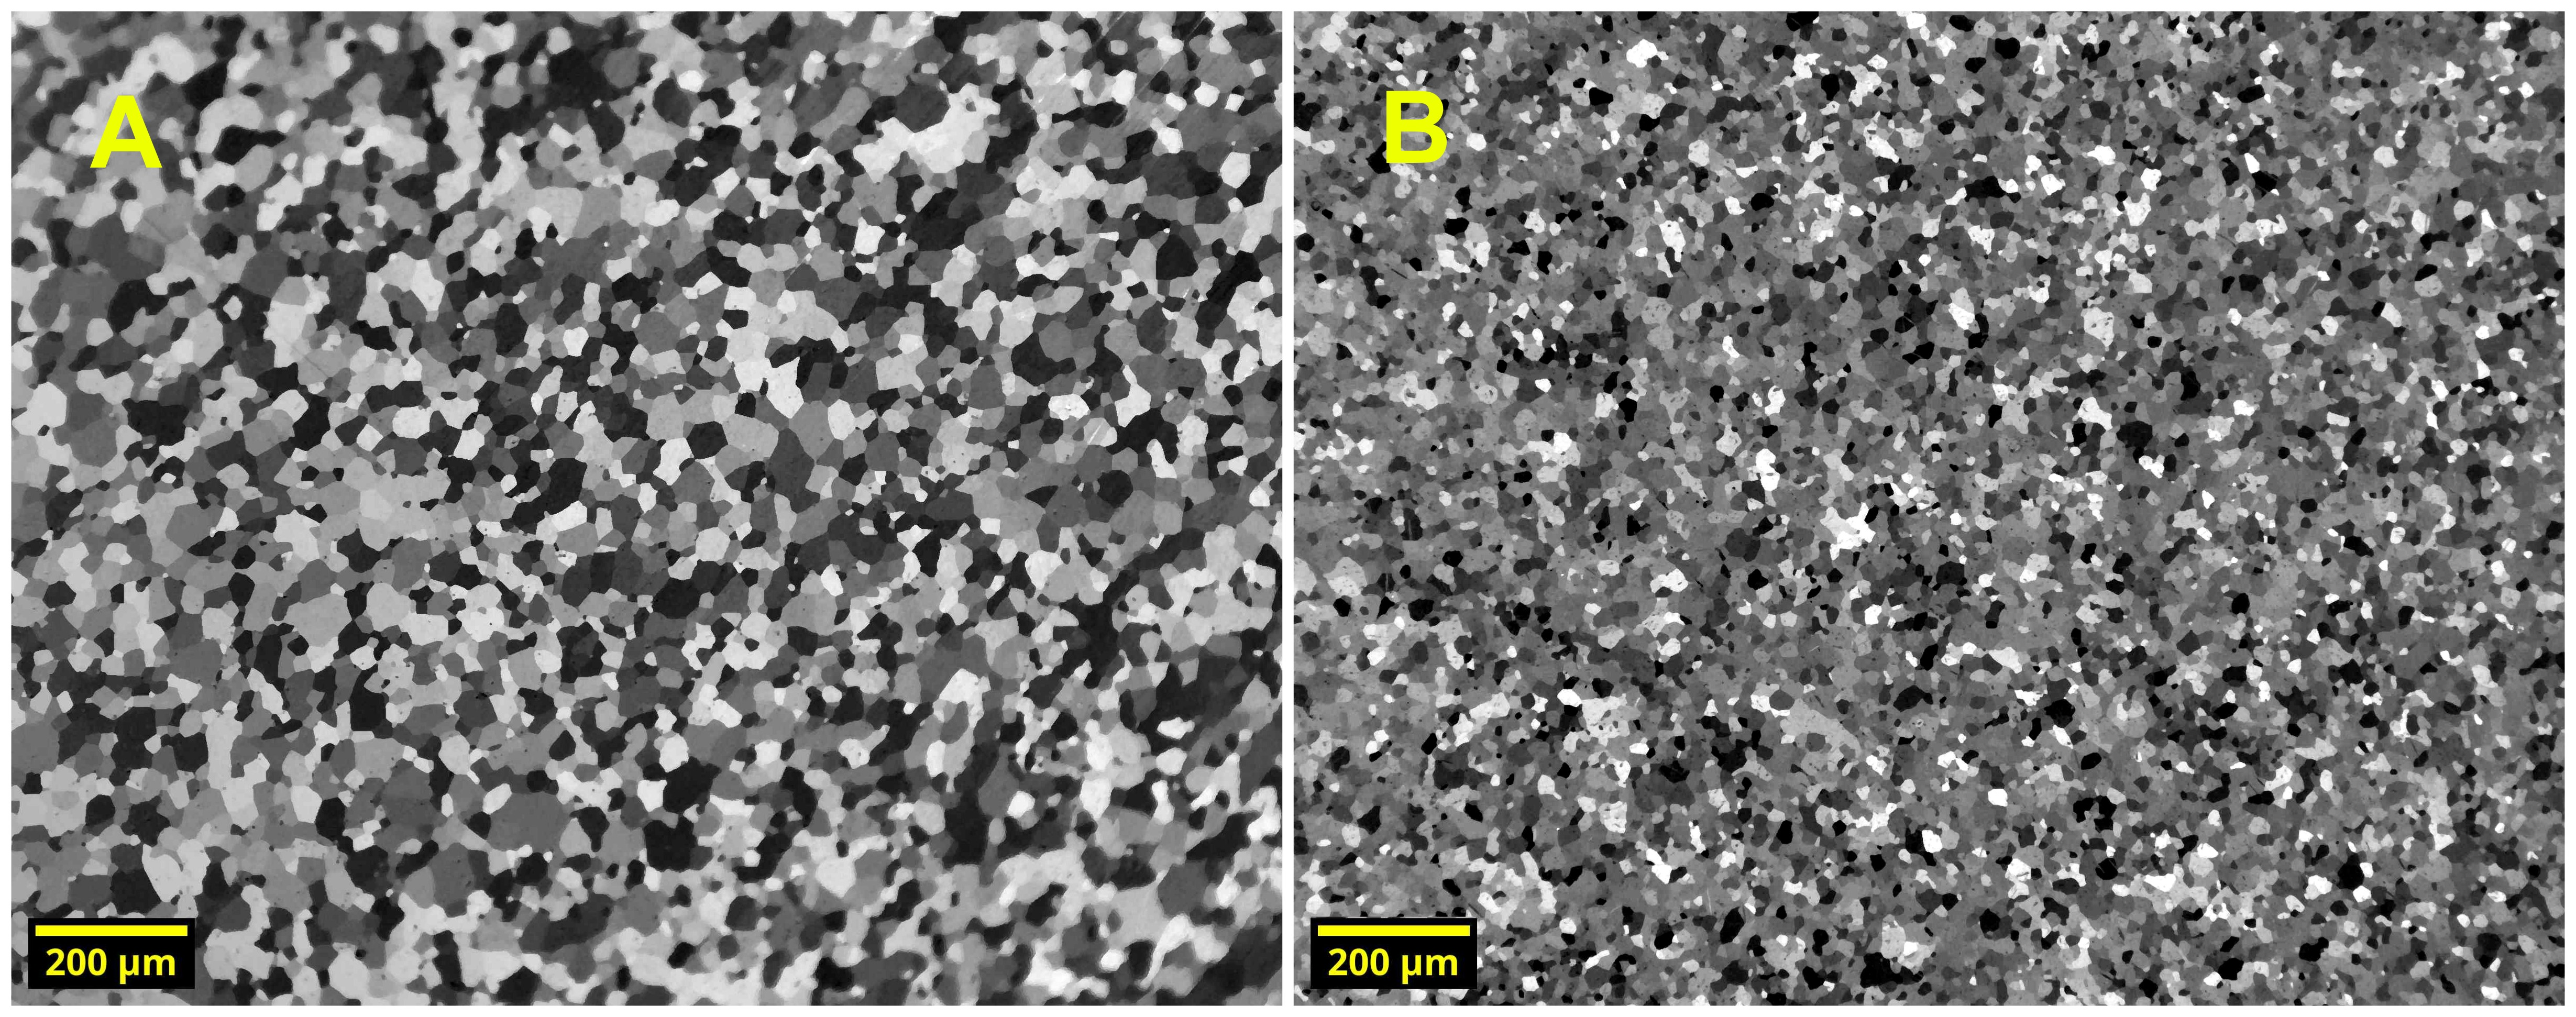
\includegraphics[width=\textwidth]{Figures/plate_sheet_OM.jpg}
  \caption{Polarised light optical micrograph of CP-Ti plate (A) and sheet (B). \label{fig.plateSheetOM}}
\end{figure}

\begin{figure}[h]
\centering
  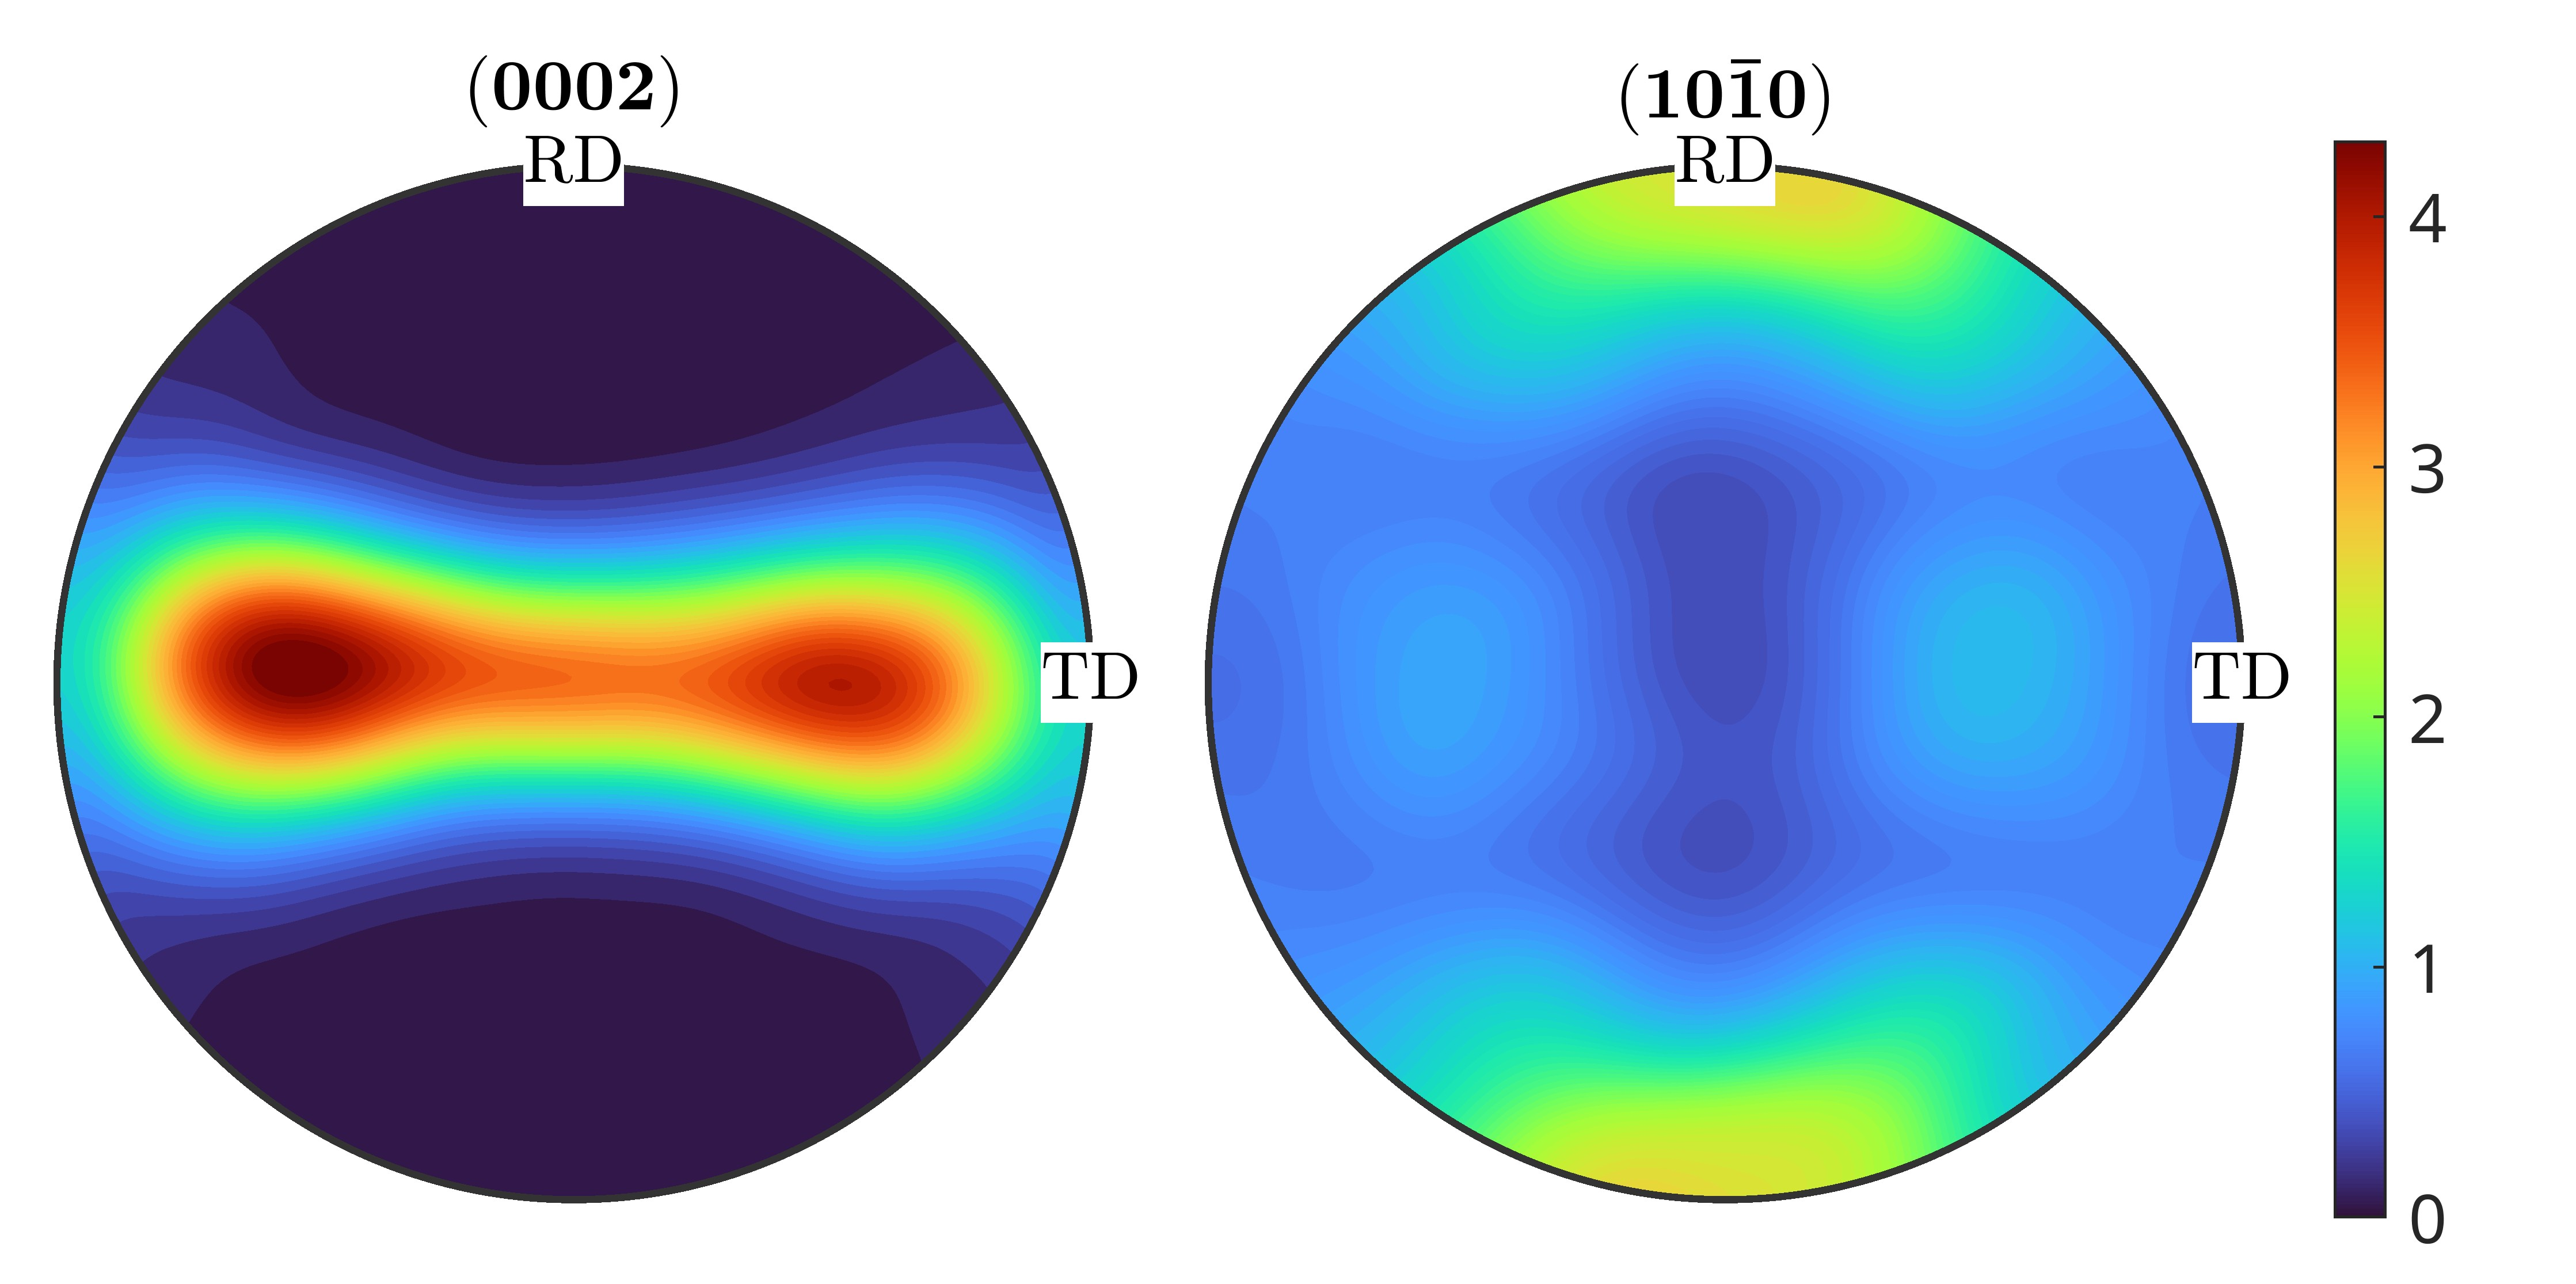
\includegraphics[width=\textwidth]{Figures/pf_plate_axisCorrectedjpg.jpg}
  \caption{Pole figures for CP-Ti plate, colour scale indicates multiples of random distribution. \label{fig.pfPlate}}
\end{figure}

Crystallographic texture measured with EBSD revealed a strong split basal texture in the CP-Ti plate, with a large TD split angle of approximately 45$^\circ$, as shown in \fref{fig.pfPlate}.
The large TD split is interesting because it exaggerates the already present anisotropy that is typical with a less pronounced TD split basal texture, with many grains having components of their $\langle c \rangle$-axis along TD but almost zero grains having $\langle c \rangle$-axis components along RD.

To examine the effect of such a strong texture, cylindrical samples along RD and TD were fabricated for tensile testing.
The results of tensile testing, shown in \fref{fig.tensilePlate}, reveal the significant anisotropy in mechanical response between the two primary plate directions.
The yield behaviour was completely different between both samples, with the RD sample undergoing a much earlier and smoother elastic-to-plastic transition.
For TD loading on the other hand, a much higher yield followed by a yield plateau was observed.

To quantify the early plasticity observed in the RD sample, the point where the stress-strain curves of the two samples diverge was determined.
The elastic limit was defined as the point when measurable plasticity in the RD sample had occurred.
The stress-strain data for both RD and TD was interpolated so that their stress difference at each strain point could be calculated by subtraction.
This difference function is plotted in \fref{fig.elasticLimit}.
During the elastic region, both samples behave very similarly and the difference remains flat.
This region was classified as the first 0.08\% strain, and the mean and standard deviation of the difference was determined.
Measurable plasticity was defined to be the point where the RD sample had deviated by more than 2 times the standard deviation, which occurred at a strain of 0.1\% and a stress of $111$MPa.

\begin{figure}[h!]
\centering
  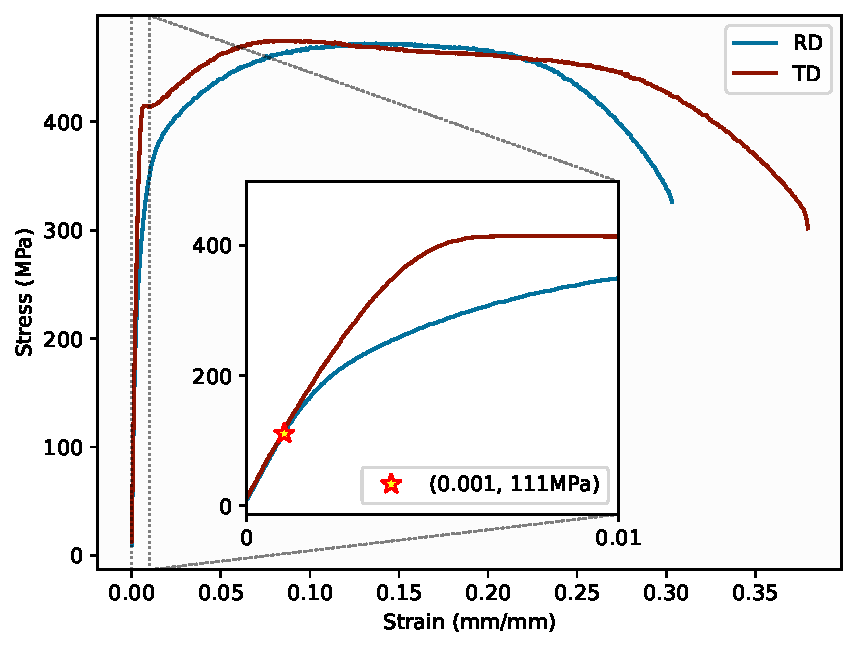
\includegraphics[width=\textwidth]{Figures/tensilePlotInset.pdf}
  \caption{Engineering stress-strain curve for CP-Ti for both rolling direction (RD) and transverse direction (TD). Elastic limit of RD sample marked on inset plot.\label{fig.tensilePlate}}
  \vspace{3\baselineskip}
  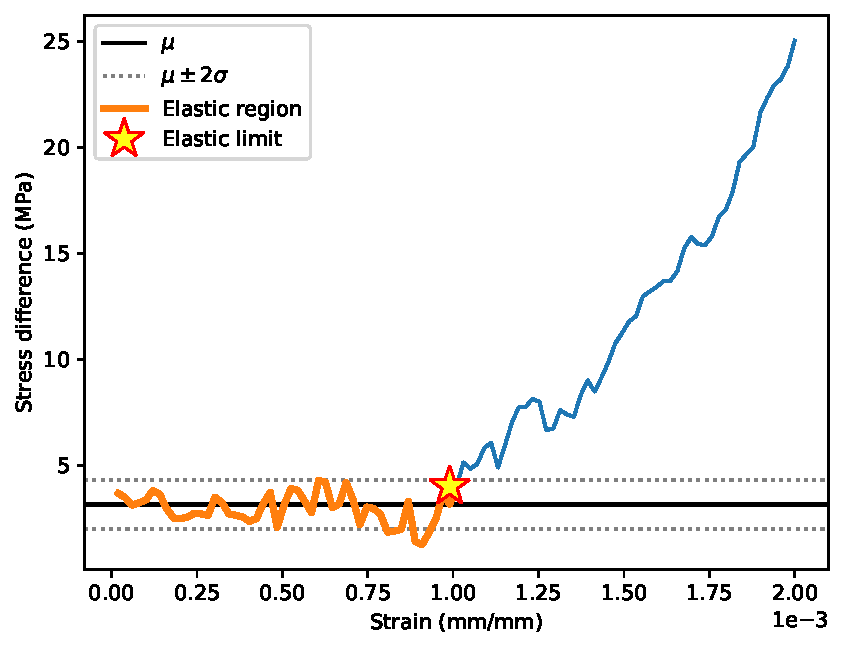
\includegraphics[width=0.6\textwidth]{Figures/elastic_limit.pdf}
  \caption{Stress difference ($\sigma_\textnormal{TD}-\sigma_\textnormal{RD}$) as a function of strain, revealing when the deformation behaviour diverges, indicating elastic limit of RD.\label{fig.elasticLimit}}
\end{figure}



\pagebreak
\section{HIP \#1: Abnormal grain growth}
The first HIP run appeared successful, and initial characterisation with EBSD revealed the desired microstructure of equiaxed $\alpha$ grains.
This initial characterisation however, was only conducted on a small part of the bottom of the HIP can.
Subsequent tensile testing results are shown in \fref{fig.tensileHIP}, in which strange load drop behaviour can be observed.
These load drops were accompanied by audible pings and were present in all 5 samples that were cut from the initial HIP can.
After some difficulty in explaining this phenomenon with respect to the assumed equiaxed microstructure, further characterisation of the material was made using cutoffs from the head sections of the tensile samples.

These cutoffs were etched using Kroll's reagent (1\% \ce{HF} + 4\% \ce{HNO3} + 95\% \ce{H2O}) and it was discovered that significant abnormal grain growth had occurred during the HIP, shown in \fref{fig.AGG}.
Very large grains can be seen which have grown to sizes on the order of several millimetres.
These grains appear to exist within a surviving matrix of normal grains which appear to be the same as the initially observed section of the HIP can, which did not present any abnormal grains.

The precise mechanism for the abnormal grain growth is not known.
It is known in the literature that the recrystallisation behaviour of alpha titanium is quite sensitive when held at high temperatures (but still beneath the beta-transus)\cite{tongFormationVeryLarge2017}.
Usually this phenomenon is related to recrystallisation after small strains, where the number density of recrystallisation nuclei may be quite small.
In such a regime, once recrystallisation nucleates, the new grain has unimpeded growth.
Provided that the small amount of work stored in the matrix is sufficient to support its growth, the new grain may grow to a very large size if there were no nearby recrystallisation nuclei.
The small strain in our case would be the initial plasticity required for consolidation of the powder.

In order to gain a deeper understanding and also as a second attempt at producing a fully random texture and consolidated HCP material, a second HIP was run using the two alternative powder stocks.
There was evidence of powder contamination in the original material, and therefore it was a plausible option to retry the same parameters with a different and hopefully uncontaminated powder.
The difference in powder size distribution would also change the dynamics of the early stage plasticity during consolidation and hopefully lead to a different result.


\begin{figure}[h]
\centering
  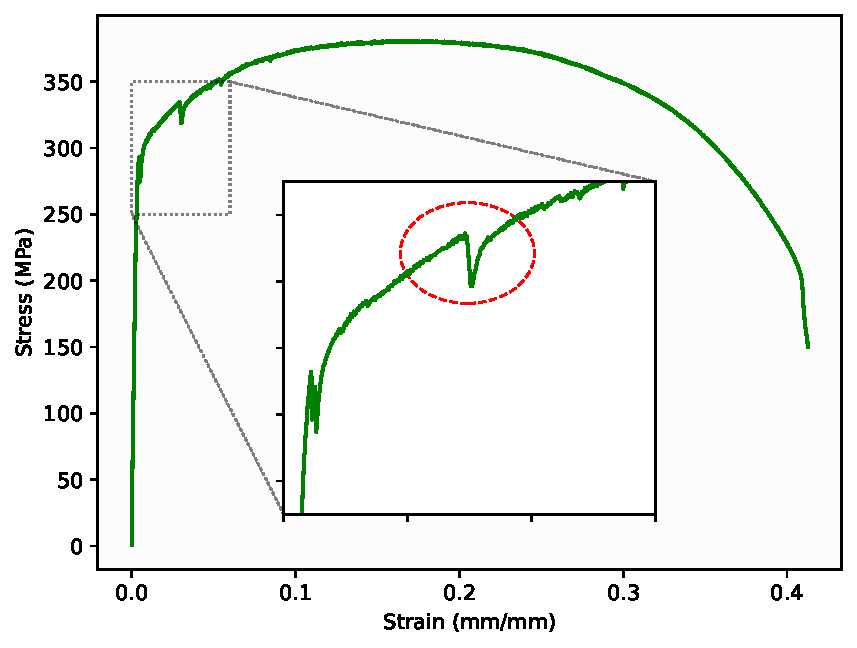
\includegraphics[width=\textwidth]{Figures/HIPtensile.pdf}
  \caption{Engineering stress-strain curve for HIP CP-Ti. Later discovered abnormal grain growth to be the cause of load drops. \label{fig.tensileHIP}}
  \vspace{\baselineskip}
  \includegraphics[width=\textwidth]{Figures/AGG.jpg}
  \caption{Optical micrograph of HIPed CP-Ti abnormal grain growth with Kroll's etch. \label{fig.AGG}}
\end{figure}


\section{HIP \#2: Success}

The second HIP trial was indeed successful, in both cases.
The two powder stocks that were used were the 45-90 $\mu$m (TLS powder) and the 53-100 $\mu$m (AVI powder). 
The resulting microstructure these cans had a grain size distribution of approximately 50 $\mu$m and 60 $\mu$m respectively (which may indicate that powder particle size is well correlated to final grain size).

The texture of the second HIP was quantified using EBSD large area measurements, which sampled many grains to generate pole figures, shown in \fref{fig.pfHIP}.
The same colour scale from \fref{fig.pfPlate} which highlights the sharp difference in texture strength.
Despite lacking any distinct texture features, the pole figure is not completely flat, which can be attributed to the sampling of a limited (though large) set of grains.

\begin{figure}[h!]
\centering
  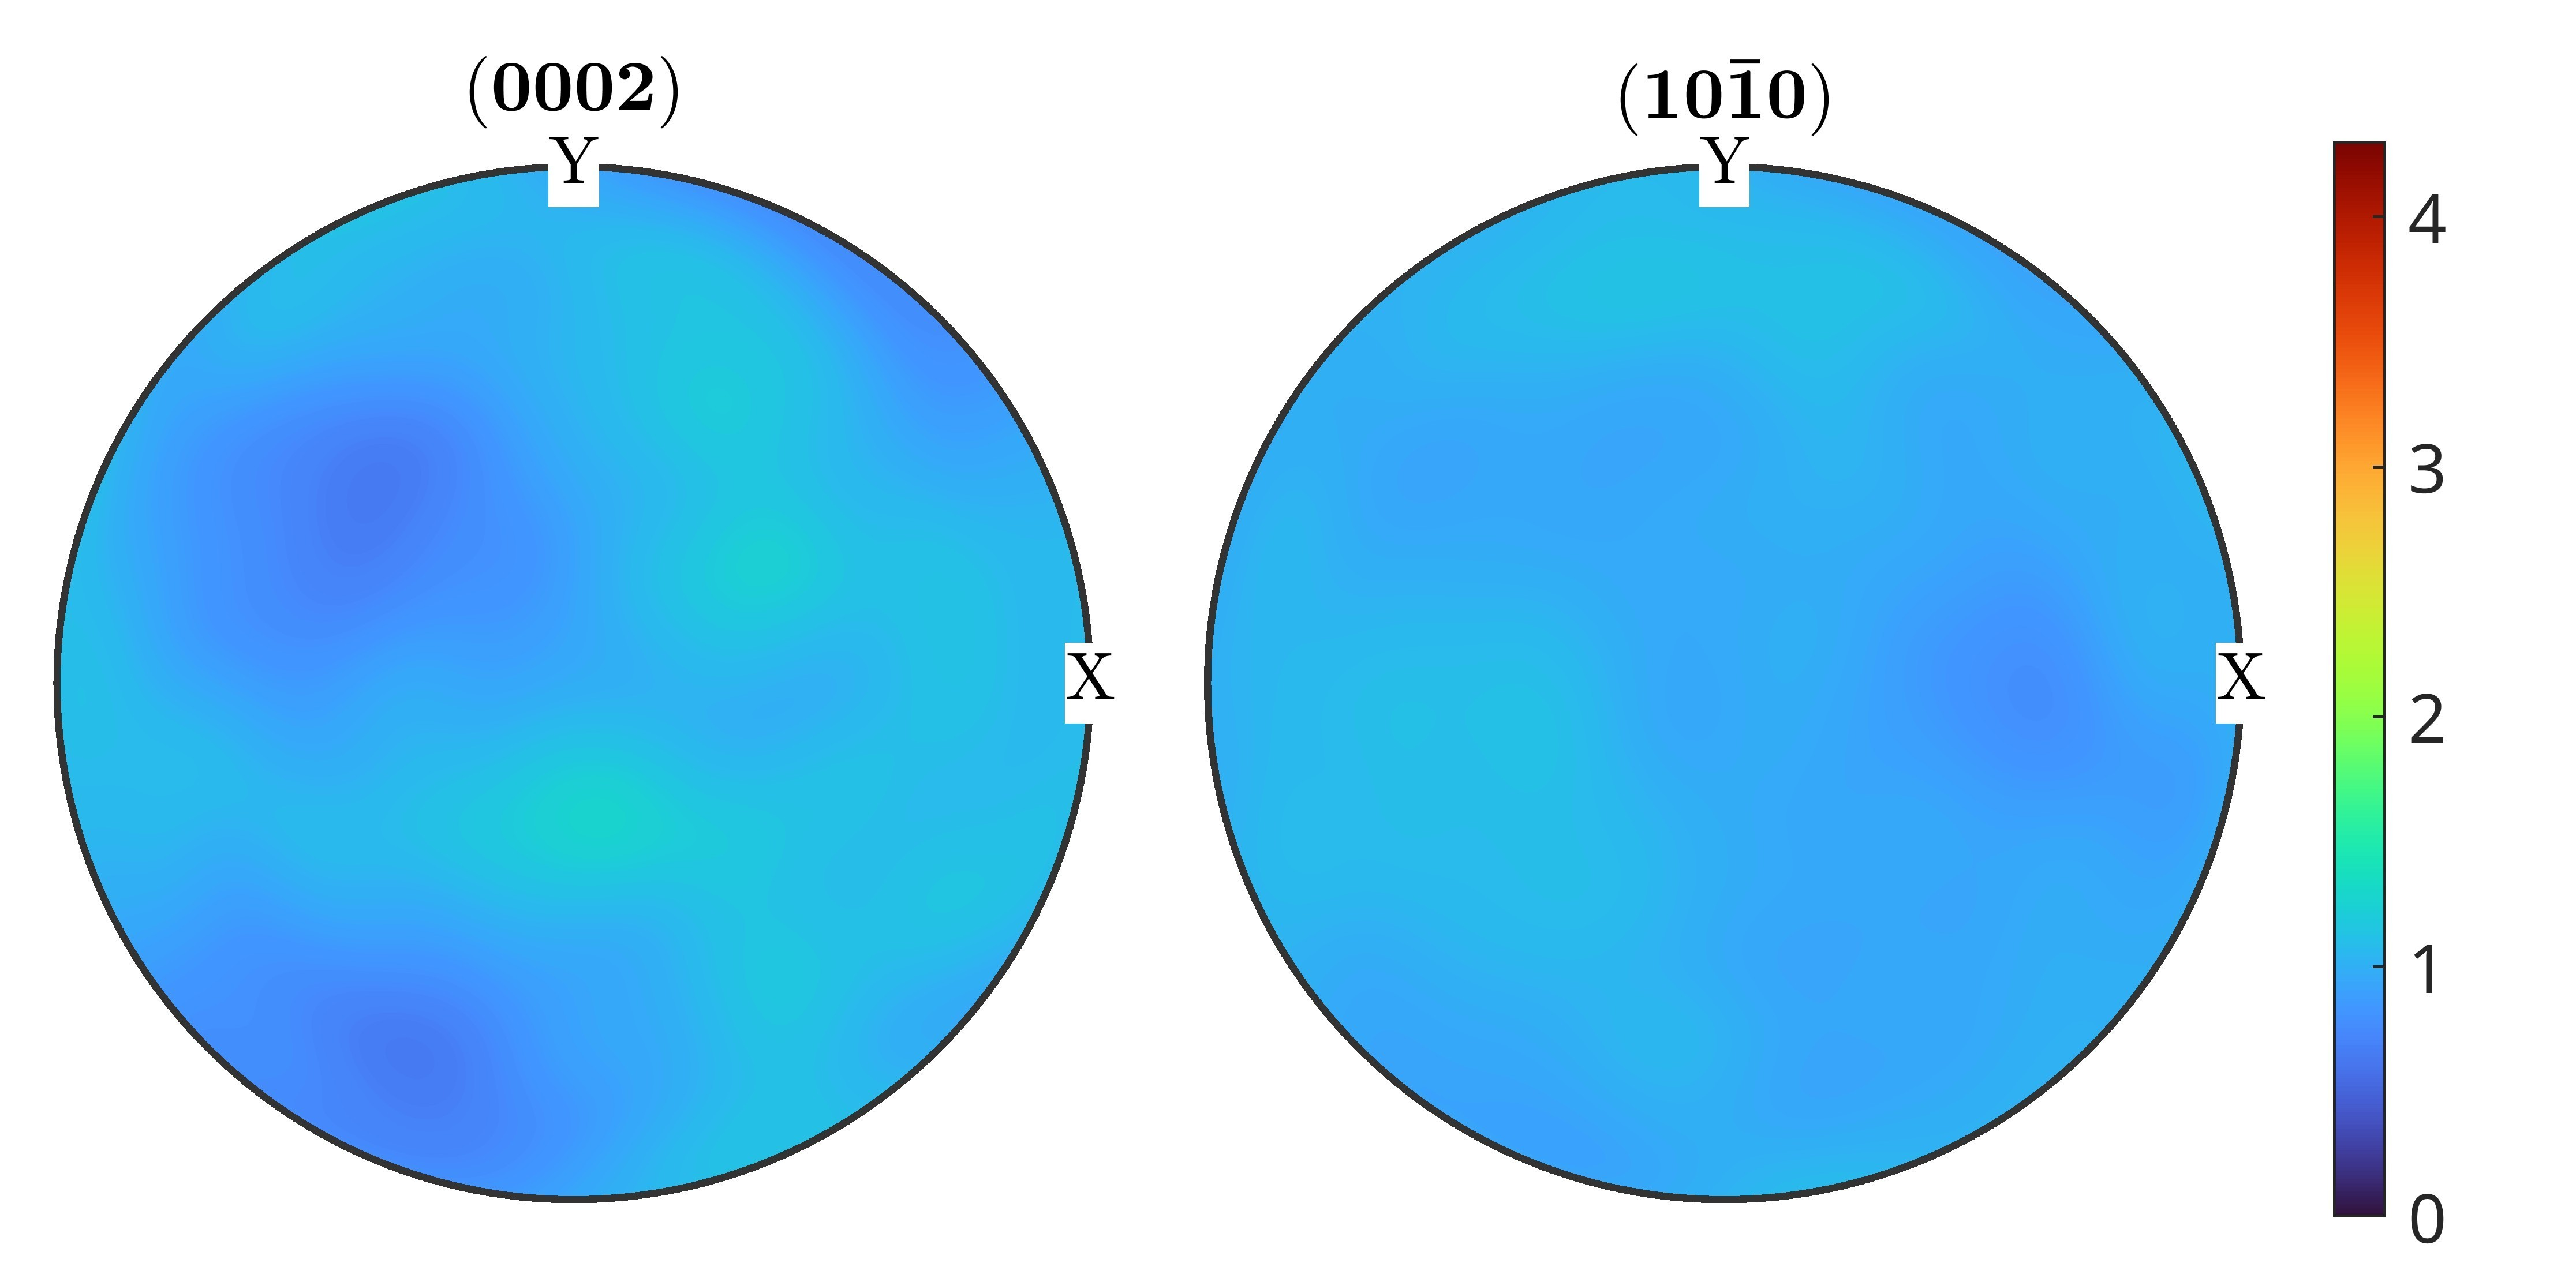
\includegraphics[width=\textwidth]{Figures/pf_HIP_TLS.jpg}
  \caption{Pole figures for HIPed CP-Ti using same colour scale as \fref{fig.pfPlate}.\label{fig.pfHIP}}
  \vspace{\baselineskip}
  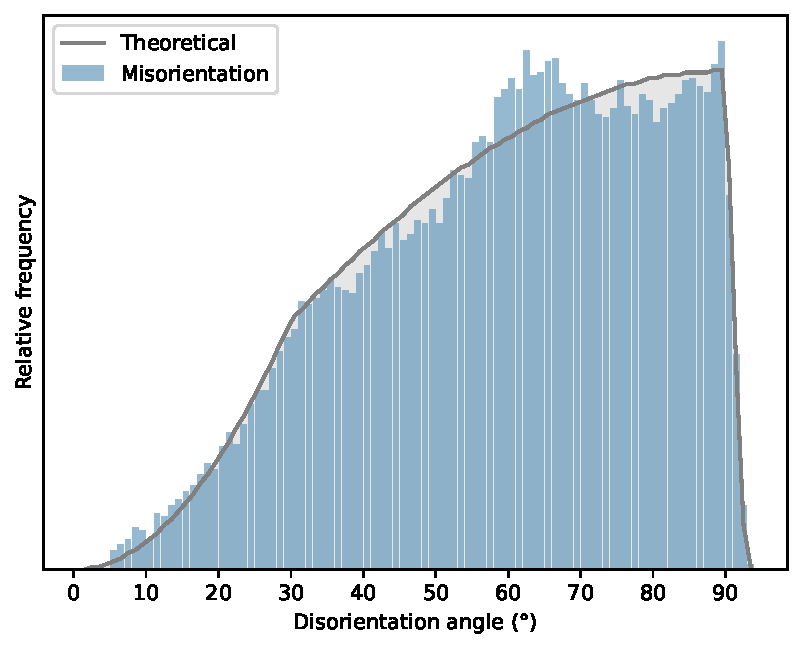
\includegraphics[width=0.7\textwidth]{Figures/disorientationDist.pdf}
  \caption{Disorientation distribution for HIP\#2, agreement with theoretical distribution for random texture.\label{fig.disorientationPlot}}
\end{figure}

The random-texture can further be quantified using the three Kearns factors: 0.3363, 0.3249, 0.3388.
For a theoretically random texture, the Kearns factors are each exactly 1/3.
Finally, the disorientation plot in \fref{fig.disorientationPlot} shows a very close agreement to the theoretical Mackenzie plot for a truly random orientation distribution.
It is therefore concluded that HIPing has proved a successful technique for producing randomly textured HCP microstructures.


\subsection{Geometric compatibility}
EBSD maps were used to calculate the grain neighbour compatibility in both the HIPed material and the conventionally rolled material.
First, a global loading condition along RD was assumed, which allowed Schmid factor analysis to be used to determine the active slip system in each grain.
Only prismatic slip systems were considered for this preliminary analysis.
Once the active slip systems were identified, for each neighbouring pair, the Luster-Morris parameter $m'$ was calculated across their boundary to determine how well the pair can accommodate slip between them.
A map of these $m'$ values in the HIP material is shown in \fref{fig.mPrimeMap}, where brighter colours represent boundaries most likely to be sites for slip transfer events.

A statistical representation of the $m'$ values is shown by the histogram in \fref{fig.mPrimeHist}.
A distinct peak at the high end of $m'$ values is present in the rolled material which is completely absent in the HIPed material.
A typical threshold for direct slip transfer is $m' > 0.8$ \cite{nieto-valeirasAnalysisSlipTransfer2024}.
In the rolled sample, 19\% fo grain boundaries are above this threshold, compared to only 7\% in the HIPed sample.
There is a measurable difference in the geometric alignment of neighbouring grains, which can be explained by the rolled texture having a more restricted set of possible grain orientations due to many orientations being absent from the orientation distribution (e.g. almost zero grains with c-axis aligned with RD).
This means that grains are more likely to have similar orientations with their neighbours and this is reflected in the peak at higher $m'$ values.

If polycrystalline strain localisation can be considered as a networking phenomenon, then a description based on percolation theory may be suitable.
The extent of networks of geometrically aligned grains would then be dependent on the expected fraction of neighbouring grains that have good alignment.


\begin{figure}[ht]
\centering
  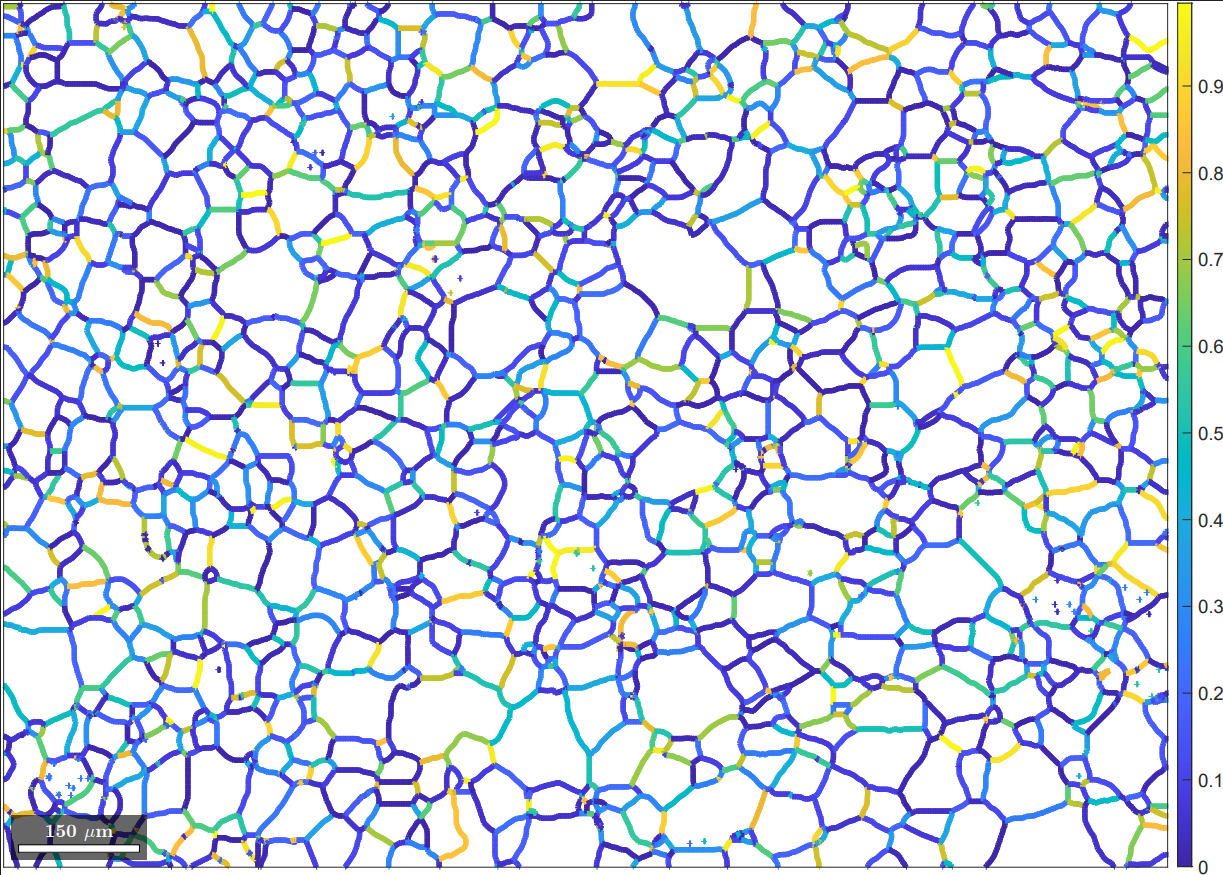
\includegraphics[width=\textwidth]{Figures/mPrimeMap_HIP.png}
  \caption{Map of $m'$ values in HIPed CP-Ti.\label{fig.mPrimeMap}}
  \vspace{\baselineskip}
  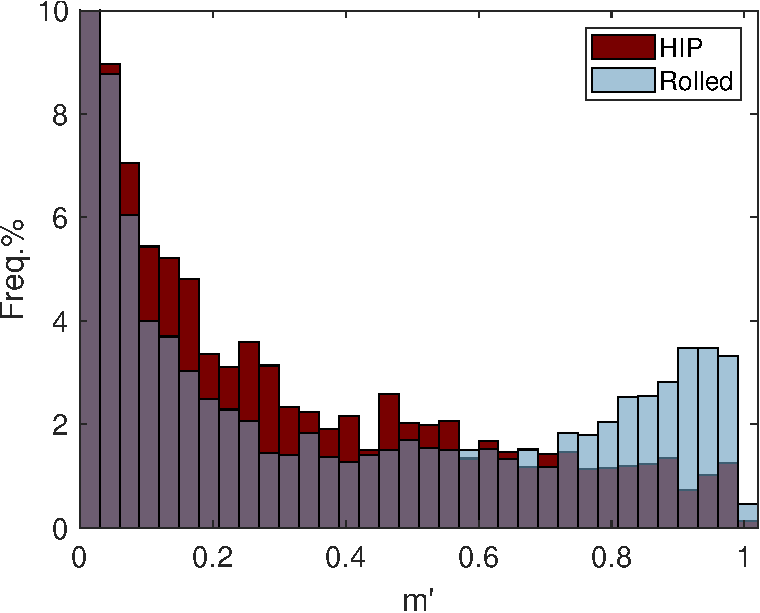
\includegraphics[width=0.8\textwidth]{Figures/mPrimeHistogram.pdf}
  \caption{Histogram of $m'$ values for rolled (RD loading) and HIPed CP-Ti.\label{fig.mPrimeHist}}
\end{figure} 

\chapter{Proposed research}

\section{Mechanical testing of HIPed material}
The most immediate next step in the project is the mechanical testing of the HIPed material.
Simple tensile tests using the same parameters as for the rolled plate samples, and using the same sample geometry.
In addition to simple uniaxial tensile testing, cycle loading tests alongside the rolled samples would allow for a comparison of the kinematic hardening behaviour between the two samples.
Post-mortem analysis of the microstructure after interrupted tensile tests would also provide insight into the role that deformation twinning plays during plasticity.

\section{HR-DIC in-situ testing}
Use of the new capability at Monash Centre for Electron Microscopy (MCEM) for in-situ tensile testing would allow for high resolution digital image correlation to be used to map the strain localisation throughout the microstructure as a function of total strain.
This technique, when paired with Relative Displacement Ratio (RDR) analysis would allow for identification of active slip modes and in-situ EBSD correlation would track the twinning behaviour as well as localised crystal rotation.

\section{Rolling HIPed material}
Direct comparison of the HIPed material to the purchased rolled plate is difficult as the exact alloy composition is not consistent, particularly the oxygen content, which has a significant effect on the mechanical properties.
To truly isolate crystallographic texture as the only independent variable, the HIPed material will be rolled to produce intermediate textures.
This will involve rolling to multiple different thickness reductions, and then calibrating a heat treatment regime for each of them to produce a recrystallised microstructure with constant grain size across all samples.
Mechanical testing and analysis of these samples would then truly highlight the transition between completely random texture to the presence of a strong crystallographic texture which is more akin to what is typically found in service.

\section{Crystal plasticity modelling}
The next stages in crystal plasticity modelling will be calibrating a twinning model to reproduce the anisotropic response from the rolled plate samples.
Once tensile data for the HIPed material is obtained, it can be incorporated into the fitting regime as an additional constraint.

Beyond this, novel constitutive behaviuour laws will be developed to incorporate a description of the geometric compatibility effect, especially in relation to long range networks of strain.
To account for complex interfacial interactions, composite voxels will be incorporated using AMITEX.

\chapter{Research communication}



%\input{Chapters/Chapter6} 

%\input{Chapters/Chapter7} 

%% ----------------------------------------------------------------
% Now begin the Appendices, including them as separate files

%\addtocontents{toc}{\vspace{2em}} % Add a gap in the Contents, for aesthetics

%\appendix % Cue to tell LaTeX that the following 'chapters' are Appendices

%\chapter{An Appendix}

Lorem ipsum dolor sit amet, consectetur adipiscing elit. Vivamus at pulvinar nisi. Phasellus hendrerit, diam placerat interdum iaculis, mauris justo cursus risus, in viverra purus eros at ligula. Ut metus justo, consequat a tristique posuere, laoreet nec nibh. Etiam et scelerisque mauris. Phasellus vel massa magna. Ut non neque id tortor pharetra bibendum vitae sit amet nisi. Duis nec quam quam, sed euismod justo. Pellentesque eu tellus vitae ante tempus malesuada. Nunc accumsan, quam in congue consequat, lectus lectus dapibus erat, id aliquet urna neque at massa. Nulla facilisi. Morbi ullamcorper eleifend posuere. Donec libero leo, faucibus nec bibendum at, mattis et urna. Proin consectetur, nunc ut imperdiet lobortis, magna neque tincidunt lectus, id iaculis nisi justo id nibh. Pellentesque vel sem in erat vulputate faucibus molestie ut lorem.

Quisque tristique urna in lorem laoreet at laoreet quam congue. Donec dolor turpis, blandit non imperdiet aliquet, blandit et felis. In lorem nisi, pretium sit amet vestibulum sed, tempus et sem. Proin non ante turpis. Nulla imperdiet fringilla convallis. Vivamus vel bibendum nisl. Pellentesque justo lectus, molestie vel luctus sed, lobortis in libero. Nulla facilisi. Aliquam erat volutpat. Suspendisse vitae nunc nunc. Sed aliquet est suscipit sapien rhoncus non adipiscing nibh consequat. Aliquam metus urna, faucibus eu vulputate non, luctus eu justo.

Donec urna leo, vulputate vitae porta eu, vehicula blandit libero. Phasellus eget massa et leo condimentum mollis. Nullam molestie, justo at pellentesque vulputate, sapien velit ornare diam, nec gravida lacus augue non diam. Integer mattis lacus id libero ultrices sit amet mollis neque molestie. Integer ut leo eget mi volutpat congue. Vivamus sodales, turpis id venenatis placerat, tellus purus adipiscing magna, eu aliquam nibh dolor id nibh. Pellentesque habitant morbi tristique senectus et netus et malesuada fames ac turpis egestas. Sed cursus convallis quam nec vehicula. Sed vulputate neque eget odio fringilla ac sodales urna feugiat.

Phasellus nisi quam, volutpat non ullamcorper eget, congue fringilla leo. Cras et erat et nibh placerat commodo id ornare est. Nulla facilisi. Aenean pulvinar scelerisque eros eget interdum. Nunc pulvinar magna ut felis varius in hendrerit dolor accumsan. Nunc pellentesque magna quis magna bibendum non laoreet erat tincidunt. Nulla facilisi.

Duis eget massa sem, gravida interdum ipsum. Nulla nunc nisl, hendrerit sit amet commodo vel, varius id tellus. Lorem ipsum dolor sit amet, consectetur adipiscing elit. Nunc ac dolor est. Suspendisse ultrices tincidunt metus eget accumsan. Nullam facilisis, justo vitae convallis sollicitudin, eros augue malesuada metus, nec sagittis diam nibh ut sapien. Duis blandit lectus vitae lorem aliquam nec euismod nisi volutpat. Vestibulum ornare dictum tortor, at faucibus justo tempor non. Nulla facilisi. Cras non massa nunc, eget euismod purus. Nunc metus ipsum, euismod a consectetur vel, hendrerit nec nunc.	% Appendix Title

%\input{Appendices/AppendixB} % Appendix Title

%\input{Appendices/AppendixC} % Appendix Title

\addtocontents{toc}{\vspace{4em}}  % Add a gap in the Contents, for aesthetics
\backmatter

%% ----------------------------------------------------------------
\label{Bibliography}
\lhead{\emph{Bibliography}}  % Change the left side page header to "Bibliography"
\bibliographystyle{unsrtnat}  % Use the "unsrtnat" BibTeX style for formatting the Bibliography
\bibliography{Bibliography.bib}  % The references (bibliography) information are stored in the file named "Bibliography.bib"

\end{document}  % The End
%% ----------------------------------------------------------------
